\chapter{Введение}
\label{chap:intro}

\section{Ассистенты доказательств}

Ассистенты доказательств, также известные как интерактивные доказательные системы (ITP),
это программные инструменты, используемые в математике, компьютерных науках и формальных методах
для помощи в разработке и проверке математических доказательств.
Эти инструменты играют важную роль в обеспечении корректности и надежности
сложных математических утверждений и программных систем.
Примеры таких инструментов включают Agda~\cite{BoveDybjerNorell2009}, Coq~\cite{BertotCasteran2013} и Lean~\cite{deMouraUllrich2021}.

Хотя проверка доказательств похожа на типизацию в языках программирования,
она обычно рассматривается как интерактивный процесс между математиком и ассистентом доказательств.
Для этого большинство ассистентов доказательств предоставляют интерактивные возможности через специализированные IDE
(например, CoqIDE\footnote{\url{https://coq.inria.fr/refman/practical-tools/coqide.html}}),
интеграцию с Proof General~\cite{Aspinall2000}, или Visual Studio Code
(через Language Server Protocol (LSP)~\cite{Gunasinghe2022}).
Большинство известных ассистентов доказательств поддерживают несколько таких опций.

\Rzk{}~\cite{Kudasov2023-github-rzk} - новый ассистент доказательств, основанный на теории типов Рила-Шулмана для синтетических $\infty$-категорий~\cite{RiehlShulman2017, Riehl2023}.
Этот экспериментальный ассистент недавно был успешно использован для формализации некоторых фундаментальных результатов для $\infty$-категорий,
включая лемму Йонеды для $\infty$-категорий~\cite{Kudasov2023}.
Однако \Rzk{} не имел многих из упомянутых интерактивных функций, таких как подсветка синтаксиса.
В этой статье мы описываем реализацию утилит и интерактивных инструментов для \Rzk{},
с акцентом на поддержку сервера языка и расширения для VS Code.
Цель - предоставить более удобный интерфейс для \Rzk{}, который будет полезен как новичкам, так и опытным пользователям.

\section{Серверы языков}

Несколько лет назад, когда появлялся новый редактор кода,
он должен был поддерживать популярные языки программирования
и зависел от плагинов, написанных специально для этого редактора, чтобы поддерживать другие языки.
Это приводило к множеству повторяющихся работ для обеспечения функций языка в разных редакторах
и к несоответствиям между функциями языка в разных редакторах.
Идея серверов языков, предложенная Microsoft, решает эту проблему,
стандартизируя протокол для общения между редактором кода (клиентом) и фоновым процессом (сервером),
предоставляющим функции языка для определенного языка. Этот протокол известен как Language Server Protocol (LSP) \cite{Gunasinghe2022}.
С LSP разработчику языка нужно реализовать сервер один раз,
и он автоматически получит поддержку языка в любом редакторе, поддерживающем LSP.
Точно так же редактор, поддерживающий LSP, автоматически получит поддержку любого языка программирования, имеющего LSP-сервер.
Примеры функций языка включают предоставление диагностических сообщений, переход к месту определения идентификатора, автозаполнение текста, семантическую подсветку синтаксиса и многое другое.

\begin{figure}
  \centering
  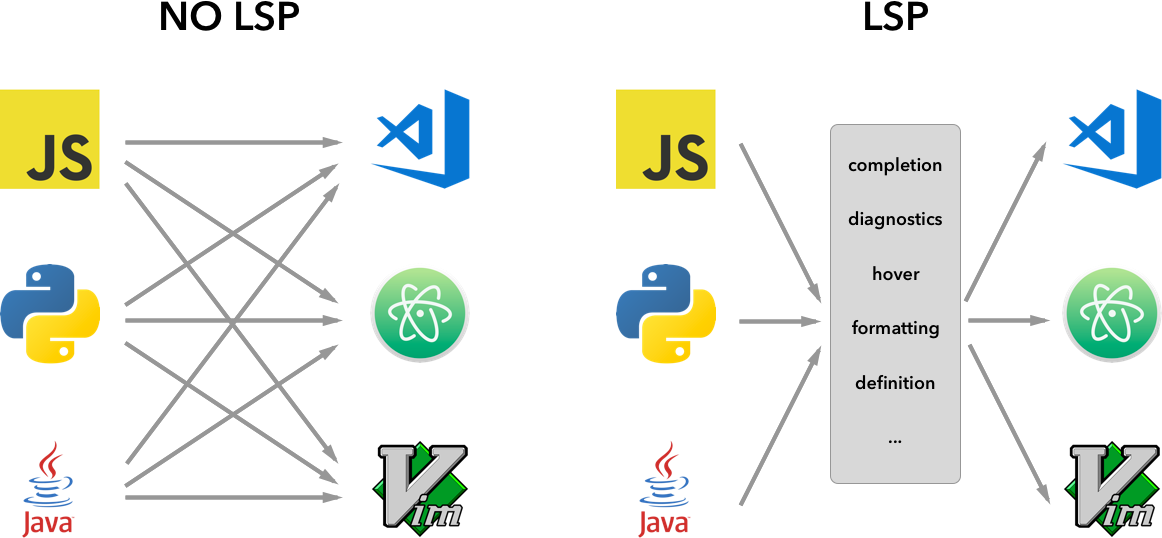
\includegraphics[width=0.7\textwidth]{figs/LSP-MxN.png}
  \label{figure:lsp}
  \caption{
    Мотивация создания LSP, с сайта Microsoft.
    \protect\footnotemark
  }
\end{figure}
\footnotetext{\raggedright\url{https://code.visualstudio.com/api/language-extensions/language-server-extension-guide}}

Этот протокол особенно полезен для интерактивных доказательных систем, поскольку
они больше зависят от удобства редактирования, чем от командной строки.
Это связано с тем, что доказательные системы не нуждаются в компиляции
в исполняемый файл и требуют только этапа проверки типов компиляторов,
который легко может быть выполнен сервером языка. Однако это также увеличивает нагрузку
на сервер языка, так как он должен поддерживать больше функций, чем обычный компилятор,
включая отображение переменных в контексте с их типами, поддержку символов Unicode
и, самое главное, возможность пошагового интерактивного доказательства.

\section{Вклад}

В этой статье мы описываем работу по реализации утилит и интерактивных инструментов для \Rzk{},
с акцентом на поддержку сервера языка и расширения для VS Code.
Ранее отчет о прогрессе этой работы был представлен на конференции PSSV 2023
в Иннополисском университете \cite{PSSV2023}.

Основные вклады включают следующее:
\begin{itemize}
  \item Сервер языка для \Rzk{}, поддерживающий основные функции LSP, такие как диагностика, автозаполнение кода и семантическая подсветка синтаксиса.
  \item Расширение для VS Code, позволяющее пользователям легко загружать и использовать сервер языка.
  \item Форматтер кода для \Rzk{}.
  \item Плагин для MkDocs, позволяющий рендерить фрагменты кода \Rzk{} в документах Markdown.
  \item Интеграция упомянутых дополнений в существующие проекты формализации \Rzk{}.
\end{itemize}
